\documentclass[11pt]{article}
\usepackage[T1]{fontenc}
\usepackage{lmodern,microtype,amsmath,amssymb,amsthm,mathtools,booktabs,array,xurl}
\usepackage[a4paper,margin=28mm]{geometry}
\usepackage{tikz}
\usetikzlibrary{arrows.meta,positioning}
\usepackage[colorlinks=true,linkcolor=blue!55!black,citecolor=blue!55!black,urlcolor=blue!55!black]{hyperref}
\setlength{\emergencystretch}{2em}
\numberwithin{equation}{section}
\newtheorem{theorem}{Theorem}[section]
\newtheorem{proposition}[theorem]{Proposition}
\newtheorem{lemma}[theorem]{Lemma}
\newtheorem{corollary}[theorem]{Corollary}
\theoremstyle{definition}\newtheorem{definition}[theorem]{Definition}
\theoremstyle{remark}\newtheorem{remark}[theorem]{Remark}
\newcommand{\ii}{\mathrm i}
\newcommand{\dd}{\mathrm d}
\newcommand{\Rea}{\operatorname{Re}}
\newcommand{\Ima}{\operatorname{Im}}
\newcommand{\Vol}{\operatorname{Vol}}
\newcommand{\diag}{\operatorname{diag}}
\newcommand{\Log}{\operatorname{Log}}
\newcommand{\stat}{\operatorname{stat}}
\newcommand{\rem}{\operatorname{rem}}
\newcommand{\Turn}{\mathsf T}
\newcommand{\CC}{\mathbb C}
\newcommand{\calC}{\mathcal C}
\newcommand{\calE}{\mathcal E}
\title{Degree and twist estimates for circle-tree invariants}
\author{}\date{}
\begin{document}\maketitle

\begin{abstract}
We prove a volume asymptotic for the original reduced invariant of an
ordered tree of crossing circles. A sufficient condition is that the sum
of \(d_v/(d_v^2+n_v^2)\), over its circles, is at most \(2^{-25}\);
here \(d_v\) is graph degree and \(n_v\) is the fixed signed crossing
power. Large degree can therefore replace large twist at a vertex.
The proof keeps the full finite Newton contraction, including its
repeated-root derivatives, and estimates all discarded indices before
forming a complex wire sum. A joint Fourier argument then controls all
charges, endpoint currents and connecting contours. Its first charge
has a nonzero coefficient through both level parities. The geometric
circle-tree theorem identifies the resulting action with the volume
of the original filled knot complement. We also give the centered
microscopic main-meridian profile, with the physical framing and
edge factors retained.
\end{abstract}

\section{The diagrams and the conclusion}\label{cta:intro}

A crossing circle is an auxiliary component bounding a disk punctured
by two main strands. Filling it restores an integer power of the
crossing in that disk's original frame. Consider the following literal
ordered construction, as in \cite[Section~1]{Geometry}. A finite tree
\(\mathcal T=(V,E)\) has at least one edge. Every vertex has its own
crossing-circle tangle \(P_v\). A rooted expression is
\begin{equation}\label{cta:word}
 W_v=\left(\prod_{w\in I_v^-}\Turn(W_w)\right)P_v
             \left(\prod_{w\in I_v^+}\Turn(W_w)\right).
\end{equation}
The lists have their specified orders. The turn rotates the whole
tangle and its disk frame; it is not just a scalar change of variable.
Choose a terminal root and the prescribed cylindrical closure. Keep
the actual strand orientations, a reduced cut on a main strand, and
zero framing. Require that the endpoint tracing gives one main
component and no internal closed component. There are no bare product
junctions. This is an input condition on the diagram, not a consequence
of the abstract graph.

Write \(r=|V|\), \(e=|E|=r-1\), and \(d_v\ge1\) for graph degree.
At vertex \(v\) the physical crossing power is \(n_v\in\mathbb Z\).
The diagram, all powers and orientations are fixed throughout.
Only the level \(N\ge3\) tends to infinity. Let \(F_N(M)\) be its
reduced zero-framed ADO invariant, with unknot value one, in the
physical convention of \cite{Meridian}. At \(M=1\) it is the reduced
Kashaev invariant of the same knot \(K_{\mathbf n}\). Put
\[
 q_N=e^{\pi\ii/N},\qquad d=N-1,\qquad M=q_N^s,\qquad |s|\le R<1.
\]
The level degree \(d\) is unrelated to \(d_v\).

Here is the quantitative hypothesis:
\begin{equation}\label{cta:sum}
 \mathfrak S=\sum_{v\in V}\frac{d_v}{d_v^2+n_v^2}\le2^{-25}.
\end{equation}
Neither the number of vertices nor the signs or relative sizes of
the fixed powers are bounded. A power can be zero when its degree is
large enough. The constants in the asymptotic and the initial level
may depend on the whole fixed diagram.

Define \(J(x)=\int_0^x\log(2\sin\pi u)\,\dd u\),
\(g(x)=J(2x)-4J(x)\), and \(G_0=g(1/4)\). Near \(t=u=0\) let
\begin{equation}\label{cta:psi-definition}
 \psi(0,0)=2G_0,\qquad
 \psi_t(t,u)=-\frac1\pi
     \operatorname{arsinh}\!\left(\tan(t/2)\cos(u/2)\right),
 \qquad\psi_u(t,u)=\psi_t(u,t).
\end{equation}
Branches continue from zero. The mixed derivatives agree, as checked
in Section~\ref{cta:edge}. Set
\[
 \Psi(\boldsymbol\tau)=\sum_{vw\in E}\psi(\tau_v,\tau_w),
 \qquad F_0=2eG_0,\qquad
 \Phi_{\boldsymbol\ell}(\boldsymbol\tau)
 =\Psi(\boldsymbol\tau)+\frac{\ii}{4\pi}
       \sum_v n_v\tau_v^2-\ii\sum_v\ell_v\tau_v .
\]
Let \(\boldsymbol\tau_*\) be the small critical point for
\(\boldsymbol\ell=\mathbf1\), and
\(\calC(\mathbf1)=\Phi_{\mathbf1}(\boldsymbol\tau_*)\).
Existence and uniqueness in the needed chart are proved below.

\begin{theorem}\label{cta:main}
For the fixed marked knot diagram above, suppose \eqref{cta:sum}.
There is a constant \(D_{\mathcal T,\mathbf n}\ne0\), independent
of the level parity, such that
\begin{equation}\label{cta:leading}
 F_N(1)=\Omega_N N^{3/2}D_{\mathcal T,\mathbf n}
            e^{N\calC(\mathbf1)}(1+O(N^{-1})),\qquad
 \Omega_N=q_N^{\,d^2(2w(D)+\sum_vn_v)/4}.
\end{equation}
Here \(w(D)\) is the oriented writhe of the original diagram and
\(|\Omega_N|=1\).
The original knot complement is hyperbolic and
\begin{equation}\label{cta:volume}
 \lim_{N\to\infty}\frac{2\pi}{N}\log|F_N(1)|
       =2\pi\Rea\calC(\mathbf1)
       =\Vol(S^3\setminus K_{\mathbf n}).
\end{equation}
Both level parities are included.
\end{theorem}

For the centered profile put
\[
 H_N(s)=\frac{\sin\pi s}{N\sin(\pi s/N)},\qquad
 A_N(s)=q_N^{(-w(D)-\sum_vn_v)s^2/2}.
\]
The value at zero is removable. For each edge let
\(x_{vw}^*=x(\tau_{*,v},\tau_{*,w})\), where the branch \(x(0,0)=1/4\)
is specified by
\begin{equation}\label{cta:wire}
 \tan^2(\pi x(t,u))
     =\frac1{1+\tan^2(t/2)+\tan^2(u/2)}.
\end{equation}

\begin{theorem}\label{cta:profile}
Under the same hypothesis, \(F_N(q_N^s)\) is nonzero on
\(|s|\le R<1\) for all sufficiently large \(N\), and uniformly there
\begin{equation}\label{cta:profile-formula}
 \frac{F_N(q_N^s)}{A_N(s)H_N(s)F_N(1)}
 =1-\frac{\pi s^2}{N}\sum_{vw\in E}\cot(\pi x_{vw}^*)
                                      +O_R(N^{-2}).
\end{equation}
Consequently the limit in \eqref{cta:volume} also holds uniformly
with \(F_N(1)\) replaced by \(F_N(q_N^s)\).
\end{theorem}

This is a microscopic statement: \(s\) is bounded while \(M=q_N^s\)
approaches one. It asserts neither an asymptotic on a fixed
\(M\)-neighborhood nor an all-orders annihilator theorem.

The finite inputs are precisely \cite[Proposition~6.1, Theorem~7.1
and Proposition~8.1]{Meridian}: full crossing polynomials and traces,
the original tree contraction, and its scalar ledger. The geometric
input is \cite[Theorem~1.1]{Geometry}. The analytic passage between
them is proved here. In particular the independently long-twist
theorem of \cite{Oscillatory} is not applicable merely from
\eqref{cta:sum}; a vertex may have \(n_v=0\).

\section{The original finite contraction and its discarded indices}
\label{cta:finite}

\subsection{Fixed coordinates and the physical factors}
Write \(\theta=\pi/N\), \(\eta=(-1)^{N-1}\), and let
\(\mathsf T_N(z)\) be the monic polynomial with
\(\mathsf T_N(t+t^{-1})=t^N+t^{-N}\). The pair algebra at a vertex
has relation \(P_\sigma=\mathsf T_N+2\cos(2\pi\sigma)\), with
\(\sigma=0,s\), or \(-s\) prescribed by its oriented pair type.
The common vector-space basis is
\begin{equation}\label{cta:basis}
 e_k(z)=S_k^{-2}\prod_{j<k}(c_j-z),\qquad
 S_k=\prod_{j=1}^k2\sin(j\theta),\qquad
 c_j=2\cos((2j+1)\theta),\quad 0\le k<N.
\end{equation}
An empty product is one. A canonical representative has degree
less than \(N\), obtained using its actual relation \(P_\sigma\).
The different relations are not identified as algebras.

The closing functional and paired edge factors are
\begin{equation}\label{cta:pairing}
 \phi_\sigma(f)=\eta N^2[z^d]\rem_{P_\sigma}f,\qquad
 \phi_\sigma(e_i e_j)=\mathbf1_{i+j=d},
\end{equation}
\begin{equation}\label{cta:edge-factor}
 W_k(s)=\prod_{j=1}^k
  \left(1-\frac{\sin^2(\pi s/N)}{\sin^2(\pi j/N)}\right),
 \qquad W_kW_{d-k}=H_N^2.
\end{equation}
Every physical turn contributes its prescribed scalar
\(\gamma_e(s)\in\{1,q_N^{s^2/2},q_N^{-s^2/2}\}\).
Lowering its index with \eqref{cta:pairing} identifies the equal
indices on the two ends of the edge and leaves
\(\gamma_e H_N/W_k\), not its reciprocal.

Let \(p_v\) be the actual crossing power, including the carrier
specified by the original oriented diagram. The exact identity
of \cite[Theorem~7.1]{Meridian} is
\begin{equation}\label{cta:exact-source}
 \begin{split}
 Z_N(s)&=\sum_{\boldsymbol k\in\{0,\ldots,d\}^{E}}
       \prod_v\phi_{\sigma_v}
           \left(p_v\prod_{e\ni v}e_{k_e}\right)
       \prod_e\gamma_e(s)\frac{H_N(s)}{W_{k_e}(s)},\\
 F_N(q_N^s)&=\vartheta_{d+s}^{-w(D)}H_N(s)Z_N(s),
 \qquad \vartheta_{d+s}=q_N^{(s^2-d^2)/2}.
 \end{split}
\end{equation}
Thus cups, caps, physical turns, negative crossings, the pivotal
closure and the one reduced cut are already fixed finite data.

On every disk \(R<1\), all factors \(H_N/W_k\) and their inverses
are bounded independently of \(N,k\). For example split the factors
in \eqref{cta:edge-factor} according to
\(\min(j,N-j)\le J\) or \(>J\). The latter logarithms are bounded
by a summable constant times \(\min(j,N-j)^{-2}\).
For fixed \(J\) the former factors have no zeros on the disk;
their endpoint limits are \(1-s^2/j^2\), also zero-free.
Compactness, including the finitely many small \(N\), gives the
bound and its inverse. The same argument applies to \(H_N\).

\subsection{Bounds that retain the first normal}
Let \(m=\lfloor d/2\rfloor\). Indices \(k\le m\) will be called
low, the others high. For a canonical polynomial use the complete
norm
\[
 \|f\|_{\mathcal J}=
 \max\{|f(c)|,\ |f'(c)|:\ c\text{ a double node of }P_0;
                 \ |f(-2)|\text{ if }N\text{ is odd}\}.
\]
The derivative at the odd simple node is absent. All first
derivatives at double nodes are retained.

\begin{lemma}\label{cta:norms}
For fixed \(R<1\), a fixed number of factors and fixed integer
crossing powers, quotient multiplication, closing, and those
crossing powers have polynomial cost in \(\|\cdot\|_{\mathcal J}\).
Uniformly in all indices,
\begin{equation}\label{cta:basis-bound}
 \|e_k\|_{\mathcal J}\le C N^A
 \begin{cases}
   \exp(Ng(k/N)),&0\le k\le m,\\
   1,&m<k<N .
 \end{cases}
\end{equation}
The constants in these statements do not depend on \(s\) in its disk.
\end{lemma}
\begin{proof}
We give the conditioning and endpoint details because ignoring
derivatives would make the high-index assertion insufficient.
The distinct complete-node polynomial is
\[
 Q_N(z)=
 \begin{cases}
  2T_{N/2}(z/2),&N\text{ even},\\
  (z+2)\{U_m(z/2)-U_{m-1}(z/2)\},&N=2m+1.
 \end{cases}
\]
Here \(T_j,U_j\) are the ordinary Chebyshev polynomials.
Its interval norm and derivatives are polynomial in \(N\).
At its roots, \(|Q_N'|\ge N/2\) in the even case and at least
\(N/2\) in the odd case: for an odd interior root \(z=2\cos t\),
\(|Q_N'(z)|=N/(2\sin(t/2))\), while \(|Q_N'(-2)|=N\).
The mean-value formula bounds each Lagrange cardinal by a
polynomial in \(N\).

For a general polynomial of degree \(<N\), interpolate its values
by \(I\) of degree \(<\deg Q_N\). Write \(f-I=Q_N h\).
The values of \(h\) at the double nodes are
\((f'(c)-I'(c))/Q_N'(c)\). These determine \(h\), whose degree
is less than their number. Use \(Q_N\) for this interpolation at
even levels and \(Q_N/(z+2)\) at odd levels; the same cardinal
bound applies. Consequently the interval norm, the complete
normal norm, and the Chebyshev coefficient sum are polynomially
equivalent. One may bound derivatives without any conditioning
assumption: a degree-\(n\) Chebyshev expansion has coefficients
at most twice its interval norm, and
\(\|T_j'(z/2)\|\le j^2/2\).

Write \(C_j(z)=(t^j+t^{-j})/2\) when \(z=t+t^{-1}\).
The product identity \(2C_iC_j=C_{i+j}+C_{|i-j|}\) makes
the coefficient sum submultiplicative. Modulo \(P_\sigma\),
\[
 C_N=-\cos(2\pi\sigma),\qquad
 \rem C_{N+j}=-2\cos(2\pi\sigma)C_j-C_{N-j}\quad(0<j<N).
\]
Iteration bounds reduction of degree at most \(hN\) by
\((2\cosh(2\pi R)+1)^h\), for fixed \(h\).
Finally \([z^d]C_d=1/2\). These facts prove the asserted
polynomial costs of multiplication and \(\phi_\sigma\).

The actual crossing polynomial and its inverse are holomorphic
through the collisions in \(|\sigma|<1\), with the normals of
\cite[Proposition~6.1]{Meridian}. On a parameter circle of radius
\(R'\in(R,1)\), \(R'\ne1/2\), Lagrange interpolation has
denominator \(\sin(2\pi\sigma)\) bounded away from zero.
Its nodes have angular imaginary part \(O_{R'}(N^{-1})\).
The divided differences of \(\mathsf T_N\) and their derivatives
on that ellipse are \(O_{R'}(N^2)\) and \(O_{R'}(N^4)\):
differentiate \(2\cos(Nt)\), with endpoint limits interpreted
by its polynomial expression. The fixed-power eigenvalues,
including negative powers, are bounded there. Thus the canonical
crossing and its first derivative have polynomial interval norm.
Holomorphy and the maximum principle extend the bound through
all collisions to the disk. The mixed orders use their actual
fixed reference crossing and the bounded scalars of the same
proposition, so they satisfy the same conclusion.

For low \(k\), all values \(e_k(c_j)\) at distinct nodes are
nonnegative and bounded by \(e_k(-2)\). Interpolation by \(Q_N\)
therefore gives \(\|e_k\|_{\mathcal J}\le N^A e_k(-2)\).
Uniform sum--integral comparison of the midpoint cosine product
and sine factorial gives
\[
 \log e_k(-2)=Ng(k/N)+O(\log N),\qquad 0\le k\le m.
\]
This remains uniform at both endpoints: removing the first and
last mesh interval leaves a smooth logarithm, while each removed
logarithmic interval contributes \(O(\log N)\).

For high \(k\), put \(l=N-k\le\lfloor N/2\rfloor\) and
\(B_j(z)=\prod_{a<j}(c_a-z)\).
Reflection \(c_{d-a}=c_a\) gives
\(B_kB_l=(-1)^N P_0\). Thus \(e_k\) vanishes at every node.
At a double node indexed by \(0\le j<\lfloor N/2\rfloor\),
its derivative is zero unless \(j<l\), and otherwise
\begin{equation}\label{cta:high-normal}
 |e_k'(c_j)|
 =\frac{S_{l-1}^{\,2}}
 {2\sin((2j+1)\theta)S_{l+j}S_{l-1-j}}.
\end{equation}
To obtain this formula, compare quadratic coefficients in
\(B_kB_l=(-1)^NP_0\), using
\(P_0''(c_j)/2=N^2/(4\sin^2((2j+1)\theta))\),
\(|B_l'(c_j)|=S_{l+j}S_{l-1-j}/(2\sin((2j+1)\theta))\),
and \(S_kS_{l-1}=N\).
The denominator ratio
\(D_j=S_{l+j}S_{l-1-j}/S_{l-1}^2\) starts at
\(2\sin(l\theta)\) and is nondecreasing, since
\[
 \frac{D_{j+1}}{D_j}
   =\frac{\sin((l+j+1)\theta)}{\sin((l-1-j)\theta)}\ge1.
\]
The two angles sum to at most \(\pi\).
Equation \eqref{cta:high-normal} is consequently at most
\(1/(4\sin((2j+1)\theta)\sin(l\theta))\le N^2/16\).
The odd simple-node value is zero. This proves \eqref{cta:basis-bound}.
\end{proof}

\subsection{Discard before forming an angular sum}
Retain \(k_e/N\in I=[1/5,3/10]\) at every edge.
Each edge index occurs in two vertex factors of
\eqref{cta:exact-source}. Lemma~\ref{cta:norms} therefore bounds
the absolute rate of an assignment by
\(2\sum_{\text{low }e}g(k_e/N)\).
Direct differentiation gives
\[
 g'(1/4)=0,\qquad
 g''(x)=-\frac{4\pi}{\sin2\pi x}\le-4\pi.
\]
Since \(g(0)=g(1/2)=0\), concavity also gives \(2G_0\ge\pi/4\).
A low index outside \(I\) loses at least \(\pi/100\) from \(F_0\);
a high index loses at least \(2G_0\).
The number of assignments is polynomial in \(N\) for the fixed tree.
We have proved the full-source estimate
\begin{equation}\label{cta:discard}
 |\text{all discarded assignments}|
       \le C_R N^A e^{N(F_0-\eta_0)},\qquad \eta_0=\pi/200.
\end{equation}
The exponent loss is independent of tree size and powers; the
prefactor and starting level are not. This argument estimates
the actual vertex traces, rather than replacing a small spectral
norm by a positive coefficient cone.

On the retained indices, the edge sums commute with the polynomial
traces. Remove only the already recorded edge scalars and put
\begin{equation}\label{cta:packet}
 \begin{split}
 K_N(t,u;s)&=\sum_{k/N\in I}e_k(-2\cos t)e_k(-2\cos u)
                         \frac{H_N(s)}{W_k(s)},\\
 B_N(\boldsymbol\tau,s)&=\prod_{vw\in E}K_N(\tau_v,\tau_w;s).
 \end{split}
\end{equation}
This is an exact polynomial in each \(-2\cos\tau_v\).
Its separate degree may be larger than \(N-1\); no such bound
is assumed in the contours below. The functional \(\phi_{\sigma_v}\)
reduces the whole polynomial in its proper relation.

\section{An exact complex edge sum}\label{cta:edge}

\subsection{The interpolation and its normalization}
We use the canonical factorial lemma
\cite[Lemma~2.1]{ConwayAnalysis}, whose statement we record.
On \(-1<\Rea z<N\),
\begin{equation}\label{cta:G}
 G_N(z)=\left(\frac{2\pi}{N}\right)^z\Gamma(z+1)
       \prod_{a\ge1}
       \frac{\Gamma(Na+z+1)}
            {\Gamma(Na-z)(Na)^{2z+1}}
\end{equation}
is holomorphic and nonzero, with positive-base powers.
It satisfies \(G_N(0)=1\), \(G_N(k)=S_k\), and
\[
 \frac{G_N(z+1)}{G_N(z)}=2\sin\frac{\pi(z+1)}N,\qquad
 G_N(z)G_N(d-z)=N,\qquad G_N(s)G_N(-s)=H_N(s)^{-1}.
\]
On every compact subset of \(0<\Rea x<1\),
\begin{equation}\label{cta:G-asymptotic}
 \log G_N(Nx)=NJ(x)+\tfrac12\Log(2N\sin\pi x)
             +\frac{\pi\cot\pi x}{12N}+O(N^{-3}).
\end{equation}
All fixed derivatives, and any fixed further inverse-power order,
are uniform on smaller compact sets. Logarithms and square roots
are continued from the positive real interval. This numbered
lemma includes the convergent product and summable Stirling proof;
no periodic factor may be inserted into \eqref{cta:G}.
For background on those classical expansions see \cite[Section~5.11]{DLMF}.

The shift equation now proves the exact interpolation needed here.
For \(u=Nt/(2\pi)\), define
\begin{equation}\label{cta:interpolant}
 \mathcal B_N(x,t)=
 \frac{G_N(d/2+u)G_N(d/2-u)}
 {G_N(d/2-Nx+u)G_N(d/2-Nx-u)G_N(Nx)^2}.
\end{equation}
At \(x=k/N\) this equals \(e_k(-2\cos t)\).
Indeed successive quotients are the original cosine numerator
and sine-factorial denominator of \eqref{cta:basis}.
The exact edge insertion is
\begin{equation}\label{cta:insertion}
 \mathcal I_N(x,s)=
 \frac{G_N(Nx)^2}{G_N(Nx-s)G_N(Nx+s)},\qquad
 \mathcal I_N(k/N,s)=\frac{H_N(s)}{W_k(s)}.
\end{equation}
The second identity follows by iterating the same shift equation
and using \(G_N(s)G_N(-s)=H_N^{-1}\).

Put
\begin{equation}\label{cta:b}
 b(x,t)=\int_0^x\Log(2\cos(2\pi v)+2\cos t)\,\dd v-2J(x).
\end{equation}
Branches start at real \(x\in I,t=0\).
On a fixed complex tube about \(I\), \eqref{cta:G-asymptotic} gives
\begin{equation}\label{cta:bulk}
 \begin{split}
 \mathcal B_N(x,t)
   &=\frac{e^{Nb(x,t)}}{2N\sin\pi x}
          (1+N^{-1}b_1(x,t)+O(N^{-2})),\\
 \mathcal I_N(x,s)
   &=1-\frac{\pi s^2}{N}\cot\pi x+O_R(N^{-2}).
 \end{split}
\end{equation}
The first correction \(b_1\) is independent of \(s\).
To check the leading constant, each argument \(d/2\pm u\)
has the shift \(-1/2\), so its square-root factor is \(\sqrt N\);
the analogous denominator factors cancel these, leaving
\((2N\sin\pi x)^{-1}\). Thus no midpoint shift has been discarded.
For the second identity use
\((\log G_N)''(Nx)=\pi\cot(\pi x)/N+O(N^{-2})\)
in the symmetric difference. All remainders are holomorphic
with uniform fixed derivatives on a smaller tube.

\subsection{The exact stationary phase and an available contour}
For \(A(x,t,u)=b(x,t)+b(x,u)\), its critical branch satisfies
\begin{equation}\label{cta:critical-wire}
 \cos(2\pi x)=\frac{1-\cos t\cos u}{2+\cos t+\cos u},
 \qquad x(0,0)=1/4.
\end{equation}
This is equivalent to \eqref{cta:wire}. It follows by writing
\(A_x=0\), squaring the products of the nonzero factors, and
choosing the branch at zero; the original unsquared equation
holds there and hence nearby.
Substitute \(z=\tan\pi v\) into the \(t\)-derivative of
\eqref{cta:b}. At its critical \(x\), the resulting logarithmic
antiderivative is
\(-\pi^{-1}\operatorname{arsinh}(\tan(t/2)\cos(u/2))\).
Thus \(\psi=\stat_x A\) is exactly \eqref{cta:psi-definition}.
In particular \(\psi\) is separately even.

We need a domain for the finite sum, not just this limiting phase.
On \(|t|,|u|\le1/4\), \(|\tan(t/2)|<0.128\); the tangent form
of \eqref{cta:critical-wire} implies
\[
 |\cos(2\pi x)|<0.017,\qquad |x(t,u)-1/4|<0.003.
\]
On \(\Rea x\in I,\ |\Ima x|\le1/50\), direct differentiation gives
\begin{equation}\label{cta:Axx}
 A_{xx}=\sum_{\xi=t,u}
 \left[-\frac{2\pi\sin2\pi x}{\cos2\pi x+\cos\xi}
                         -2\pi\cot\pi x\right],
 \qquad |A_{xx}|<44,\quad \Rea A_{xx}<-12.
\end{equation}
Here are sufficient elementary bounds: \(|\cos2\pi x|<0.338\),
\(|\cos\xi-1|<0.032\), \(|\sin2\pi x|<1.009\), and
\(\Rea\cot\pi x>0.72\).
The real part of
\(\sin2\pi x/(\cos2\pi x+\cos\xi)\) exceeds \(0.328\):
its conjugated numerator is at least
\(0.95(0.655)-0.040(0.159)\), and its squared denominator is
at most \(1.37^2\). These also prove the modulus bound.

Enclose precisely the retained integers \(k\) by a rectangle in
the \(x\)-plane with vertical half-grid sides and horizontal
height \(h=1/500\). The residue formula with
\(\pi N\cot(\pi Nx)\) equals the finite sum exactly.
On a vertical half-grid side the cotangent has modulus at most
one. On horizontal sides it equals \(\mp\ii+O(e^{-2\pi Nh})\).
If \(X=\Rea(x-x_*),Y=\Ima(x-x_*)\), Taylor's formula and
\eqref{cta:Axx} imply
\begin{equation}\label{cta:contour-bound}
 \Rea\{A(x)-A(x_*)\}\le-6X^2+44|XY|+22Y^2.
\end{equation}
On a vertical side, for all large \(N\),
\(|X|\ge0.047-o(1)\) and \(|Y|\le0.005\);
the right side is below \(-0.002+o(1)\).
On a horizontal side its maximum in \(X\) is at most
\((308/3)Y^2\le77/30000\), less than
\(2\pi h=\pi/250\). All nonconstant cotangent modes and
vertical currents therefore have a fixed exponential loss
relative to \(e^{N\psi}\).

The constant horizontal terms give \(N\) times a real integral.
Translate this integral to the real tangent through \(x_*\).
Its endpoint connectors have the same loss, and
\(\Rea A_{xx}<-12\) gives a nondegenerate Gaussian. The
ordinary Taylor proof of the saddle expansion applies uniformly:
outside a fixed small saddle interval there is a fixed loss;
inside it put \(x-x_*=N^{-1/2}z\), expand, and integrate
the Gaussian-dominated remainder. Odd terms integrate to zero.
This also gives any fixed order and its parameter derivatives.
All Gamma arguments in \eqref{cta:interpolant} stay in regular
bulk strips throughout these contours.

It follows that
\begin{equation}\label{cta:edge-expansion}
 \begin{split}
 K_N(t,u;0)&=N^{-3/2}a_e(t,u)e^{N\psi(t,u)}
                     (1+N^{-1}a_{e,1}(t,u)+O(N^{-2})),\\
 a_e&=\frac{\sqrt{2\pi}}
       {4\sin^2(\pi x_*)\sqrt{-A_{xx}(x_*,t,u)}} .
 \end{split}
\end{equation}
The square root is positive at zero and continued on the disk;
no factor vanishes there. In particular \(a_e(0,0)=1/4\).
Applying the same contour to \eqref{cta:insertion} proves
\begin{equation}\label{cta:packet-expansion}
 \begin{split}
 B_N(\boldsymbol\tau,0)&=
   N^{-3e/2}a(\boldsymbol\tau)e^{N\Psi(\boldsymbol\tau)}
           (1+N^{-1}a_1(\boldsymbol\tau)+O(N^{-2})),\\
 \frac{B_N(\boldsymbol\tau,s)}{B_N(\boldsymbol\tau,0)}
   &=1-\frac{\pi s^2}{N}\sum_{vw\in E}
             \cot(\pi x(\tau_v,\tau_w))+O_R(N^{-2}),
 \qquad a=\prod_e a_e .
 \end{split}
\end{equation}
For a holomorphic insertion, its first saddle correction is
\(O(N^{-1})\), since the linear Gaussian term is odd.
Multiplication by its prefactor \(1/N\) in
\eqref{cta:bulk} therefore makes the last remainder \(O(N^{-2})\).
The common \(a_1\) cancels in this ratio.

\section{Angular bounds and weighted curvature}\label{cta:angular}

\subsection{A bound on the entire real angular period}
Let \(N\ge160\), \(k/N\in I\), and
\(r_j=\cos((2j+1)\pi/N)\). The exact product is
\[
 \frac{e_k(-2\cos z)}{e_k(-2)}
   =\prod_{j<k}Q_{r_j}(z),\qquad
 Q_r(z)=\frac{r+\cos z}{1+r}.
\]
Reserve the first \(m_0=\lfloor N/32\rfloor\) factors, where
\(r_j>\cos(\pi/16)>9/10\).
There are at most \(N/20+1\) negative parameters, all \(>-2/5\).
Pair them injectively with parameters among the next
\(N/20+1\) positions, which are \(>7/10\); these positions
are disjoint from the negative ones since \(m_0+N/20+1\le N/8\).
All remaining unpaired parameters are nonnegative.

For a pair \(r>-2/5,s>7/10\), the coefficients of
\[
 (z^2+2rz+1)(z^2+2sz+1)
\]
are \(1,2(r+s),2+4rs,2(r+s),1\), all positive.
Normalized at \(z=1\), with its central Laurent power removed,
it is a symmetric probability measure on
\(\{-2,-1,0,1,2\}\).
A remaining single factor has the analogous interpretation
on \(\{-1,0,1\}\). Its complex-angular modulus is at most
\(\cosh(by)\le e^{b^2y^2/2}\), where \(b\) is its Laurent degree.

For a reserved factor, put \(w=\sin^2(t/2)\). The two linear
pieces of \(|1-2w/(1+r)|\) give
\(|Q_r(t)|\le1-w/2\). For \(|y|\le1/4\),
\[
 |r+\cos(t+\ii y)|^2
 =(r+\cos t)^2+2r\cos t(\cosh y-1)+\sinh^2 y .
\]
Since \(2(\cosh y-1)+\sinh^2y\le4y^2\), each reserved
factor is bounded by \(\exp(-w/4+2y^2)\).
Use \(m_0\ge N/40\), then multiply the paired and reserved
estimates:
\begin{equation}\label{cta:raw}
 \left|\frac{e_k(-2\cos(t+\ii y))}{e_k(-2)}\right|
 \le\exp N\left(-\frac{\sin^2(t/2)}{160}+4y^2\right).
\end{equation}
This pairing precedes absolute values. Individual Laurent
factors need not have nonnegative coefficients.

Set \(a_v=d_v/(2\pi)\). On \(|t_v|\le\pi,\ |y_v|\le1/4\),
\(\sin^2(t_v/2)\ge t_v^2/\pi^2\), so \eqref{cta:raw},
the bounded edge insertions, and the positive zero-angle sum give
\begin{equation}\label{cta:global-Gaussian}
 |B_N(\mathbf t+\ii\mathbf y,s)|
 \le C_RN^A\exp N\left\{
 F_0-\frac1{400}\sum_va_vt_v^2+70\sum_va_vy_v^2\right\}.
\end{equation}
The stronger incidence constants are \(1/(80\pi)>1/400\)
and \(8\pi<70\).
Endpoint translations \(O_R(N^{-1})\) and derivatives cost
only polynomial factors for the fixed tree; one may apply
Cauchy's formula on radius \(1/N\) disks. This is a bound on
the entire angular period, not only near its maximum.

\subsection{The local nonlinear terms}
With
\(Q=\sqrt{1-\sin^2(t/2)\sin^2(u/2)}\), differentiation gives
\begin{equation}\label{cta:edge-Hessian}
 \psi_{tt}=-\frac{\cos(u/2)}{2\pi\cos(t/2)Q},\qquad
 \psi_{tu}=\frac{\sin(t/2)\sin(u/2)}{2\pi Q},\qquad
 \det\psi''=\frac1{4\pi^2}.
\end{equation}
Consequently
\[
 \Psi=F_0-\frac12\sum_v a_v\tau_v^2+\calE(\boldsymbol\tau).
 \]
On the polydisk \(|\tau_v|\le1/4\), put
\(\delta=1/50,\ \varepsilon=1/25\). Then
\begin{equation}\label{cta:error}
 \left|\frac{\calE_v}{\tau_v}\right|\le\delta a_v,\qquad
 \sum_w|\calE_{vw}|\le\varepsilon a_v,\qquad
 |\calE|\le\frac{\varepsilon}{2}\sum_v a_v|\tau_v|^2 .
\end{equation}
The quotient extends at zero by separate evenness.
For explicit bounds write
\(k=\cosh(1/8)-1<0.008\), \(\sigma=\sinh(1/8)<0.126\),
and \(C=(1-\sigma^4)^{-1/2}\).
The normalized diagonal error in \eqref{cta:edge-Hessian}
is at most \(2kC/(1-k)+C-1<1/50\), and the off-diagonal
bound is \(\sigma^2C\); their sum is \(<1/25\).
Summing over incident edges proves the row estimate.
Integrate the diagonal error while fixing the other variables
to prove the first estimate. For the last, sum the edge
quadratic forms and use \(2|zw|\le|z|^2+|w|^2\).
No estimate grows with the number of vertices.

\section{Critical points with degree in the denominator}
\label{cta:critical}

Set
\begin{equation}\label{cta:D}
 b_v=\frac{n_v}{2\pi},\qquad D_v=a_v-\ii b_v,\qquad
 t_0=\frac1{16},\qquad L_v=\lfloor t_0|D_v|\rfloor .
\end{equation}
The summed condition implies
\(\sqrt{d_v^2+n_v^2}\ge2^{25/2}\sqrt{d_v}\), so
\(|D_v|>32\) and \(L_v\ge1\). This denominator stays large
also when \(n_v=0\).

For real continuous charges \(0\le\ell_v\le L_v\), the critical
equation of \(\Phi_{\boldsymbol\ell}\) is
\begin{equation}\label{cta:fixedpoint}
 D_v\tau_v=-\ii\ell_v+\calE_v(\boldsymbol\tau).
\end{equation}
After division by \(D_v\), its right side is a contraction
with constant at most \(\varepsilon\) in the radius-\(1/4\)
polydisk, by \eqref{cta:error} and \(a_v\le|D_v|\).
Its image has radius at most \(t_0+\delta/4<1/4\).
It has a unique analytic critical branch
\(\boldsymbol\tau_{\boldsymbol\ell}\). Define
\(\calC(\boldsymbol\ell)=
\Phi_{\boldsymbol\ell}(\boldsymbol\tau_{\boldsymbol\ell})\).

Put \(Q_v=\calE_v/\tau_v\), with its holomorphic removable
extension. The exact equation is
\begin{equation}\label{cta:tau-formula}
 \tau_v=-\frac{\ii\ell_v}{D_v-Q_v}.
\end{equation}
Since \(|Q_v|\le\delta a_v\), define
\[
 \gamma_+=\frac{1+\delta}{(1-\delta)^2}
          =\frac{2550}{2401},\qquad
 \gamma_-=\frac{1-\delta}{(1+\delta)^2}
          =\frac{2450}{2601}.
\]
Taking the imaginary part of \eqref{cta:tau-formula} gives
\begin{equation}\label{cta:imaginary}
 \gamma_-\frac{\ell_va_v}{|D_v|^2}
 \le-\Ima\tau_v
 \le\gamma_+\frac{\ell_va_v}{|D_v|^2}.
\end{equation}
For example the numerator is
\(\ell_v\Rea(D_v-Q_v)\), between
\((1-\delta)\ell_va_v\) and \((1+\delta)\ell_va_v\);
the denominator is bounded by
\((1\pm\delta)^2|D_v|^2\).
Every positive-charge coordinate therefore has negative
imaginary part and is nonzero.

The envelope derivative is
\(\partial_{\ell_v}\Rea\calC=\Ima\tau_v\).
Integrating it one coordinate at a time gives
\begin{equation}\label{cta:charge-order}
 \Rea\calC(\boldsymbol\ell)\le\Rea\calC(\mathbf1)
   -\frac{\gamma_-}{2}\sum_v
       \frac{a_v}{|D_v|^2}(\ell_v^2-1),
 \qquad 1\le\ell_v\le L_v .
\end{equation}
Integrating from \(\mathbf0\) to \(\mathbf1\) similarly gives
\begin{equation}\label{cta:drop}
 F_0-\beta\le\Rea\calC(\mathbf1)\le F_0,\qquad
 \beta=\frac{\gamma_+}{2}\sum_v\frac{a_v}{|D_v|^2}
                         =\pi\gamma_+\mathfrak S.
\end{equation}
This compares each charge directly with the filled first-charge
action; a comparison only with \(F_0\) would not suffice.

The real part of the Hessian on a real tangent is at most
\(-(1-\varepsilon)\diag(a_v)\), by the symmetric weighted
row bound in \eqref{cta:error}. Its Gaussian determinant
is nonzero. Also
\(|\tau_v|\le t_0/(1-\delta)<\pi/2\), so
\(\prod_v\sin\tau_v\ne0\) at every positive-charge saddle.

\section{The entire Fourier filling calculation}\label{cta:Fourier}

\subsection{A translated finite grid, including its endpoint currents}
For an even trigonometric polynomial
\(f(t)=f^\sharp(-2\cos t)\), define the exact trace
\(\mathcal D_{n,\sigma,N}[f]=\phi_\sigma(R_\sigma^n f^\sharp)\).
There is no restriction on the degree of \(f^\sharp\).
The actual crossing formula of
\cite[Proposition~6.1 and equation~(6.4)]{Meridian} gives
\begin{equation}\label{cta:trace}
 \mathcal D_{n,\sigma,N}[f]
 =\frac{\eta N C_{N,n}(\sigma)}{\sin(2\pi\sigma)}
   \sum_{j=0}^{N-1}
     \sin\tau_j\, f(\tau_j)e^{\ii nN\tau_j^2/(4\pi)},
 \quad
 \begin{cases}
 \tau_j=\dfrac{2\pi}{N}(d/2+\sigma-j),\\
 C_{N,n}(\sigma)=q_N^{n(d^2/4-\sigma^2/2)} .
 \end{cases}
\end{equation}
It is initially written off the colliding grids. Its holomorphic
limit is the full trace, including first normals and the odd
simple-node value; it is not a distinct-node approximation.

Fix \(R<R'<1\), with \(R'\ne1/2\), and first put the formal
parameters \(\sigma_v\) on \(|\sigma_v|=R'\).
Their denominators are then bounded away from zero.
The grid kernel
\[
 \mathcal K_\sigma(t)=
 \frac{\ii N e^{\ii Nt}}{e^{\ii Nt}-\eta e^{2\pi\ii\sigma}}
\]
has residue one at each grid point. Integrate it around the
rectangle with sides \(\pm\pi\pm\ii y+2\pi\sigma/N\).
It encloses exactly the \(N\) points in \eqref{cta:trace}.
On its vertical sides,
\[
 \mathcal K_\sigma(\pm\pi+\ii v+2\pi\sigma/N)
           =\frac{\ii N e^{-Nv}}{1+e^{-Nv}}.
\]
Thus no argument-dependent pole separation is assumed.
The upper and lower horizontal expansions are respectively
\[
 -\ii N\sum_{\ell\ge1}
     \eta^\ell e^{-2\pi\ii\ell\sigma}e^{\ii\ell Nt},
 \qquad
 \ii N\left(1+\sum_{\ell\ge1}
     \eta^\ell e^{2\pi\ii\ell\sigma}e^{-\ii\ell Nt}\right).
\]
Each term has an entire integrand, so its translated path can
be moved to the fixed horizontal segment, retaining the short
endpoint connectors. This is not a deformation of a meromorphic
kernel through its moving poles.

The function \(\sin t\,f(t)e^{\ii nNt^2/(4\pi)}\) is odd.
Reflect the upper side by \(t\mapsto-t\), with its actual
boundary orientation. Combining the two coefficients leaves
\[
 c_{\ell,N}(\sigma)=
   \eta^{\ell-1}U_{\ell-1}(\cos2\pi\sigma),\qquad c_{1,N}=1.
\]
The zero-mode integral on the real segment is zero, but moving
it there leaves its endpoint currents. The resulting
nonzero-charge prefactor is \(-N^2C_{N,n}/(\pi\ii)\).
In particular the reflected charges have already been paired;
there will be no later unexamined sum of equal-action signs.

\subsection{Infinite tails with real spectators}
Let \(A_0=1/400\), and use the heights
\begin{equation}\label{cta:height}
 y_v=A_0t_0\,\frac{a_v}{|D_v|}.
\end{equation}
In coordinate \(v\), with all spectators real or on their
physical translated grids, \eqref{cta:global-Gaussian} bounds
the exponent on the lower horizontal side by
\[
 F_0-A_0a_v t^2+|b_vty_v|-\ell y_v+70a_vy_v^2.
 \]
After maximizing \(t\), the positive quadratic coefficient
of \(y_v^2\) is at most
\[
 70a_v+\frac{100b_v^2}{a_v}
                  \le\frac{100|D_v|^2}{a_v}.
 \]
Since \(L_v+1>t_0|D_v|\), every \(\ell\ge L_v+1\) loses at least
\begin{equation}\label{cta:tail-loss}
 \tfrac12 A_0t_0^2a_v\ge\frac1{409600\pi}.
\end{equation}
Further charges carry \(e^{-N(\ell-L_v-1)y_v}\).
The bound
\(|c_{\ell,N}(\sigma)|\le
\ell e^{2\pi R'(\ell-1)}\) is absorbed for sufficiently large
\(N\), since this tree and \(y_v>0\) are fixed.

The original vertical sides have loss
\(\pi^2a_v/400\).
The chirp, finite-charge connector and imaginary Gaussian
costs there are at most
\(\pi A_0t_0a_v\), \(A_0t_0^2a_v\), and
\(70A_0^2t_0^2a_v\). Their sum is less than half that
endpoint loss. The zero-mode current obeys the same estimate.
The translated-grid error \(O(N^{-1})\) changes only the
prefactor.

For completeness, define the finite real-integral functional
\[
 \mathcal P_v[f]=-\frac{N^2C_{N,n_v}(\sigma_v)}{\pi\ii}
   \sum_{\ell=1}^{L_v}c_{\ell,N}(\sigma_v)
   \int_{-\pi}^{\pi}\sin t\,f(t)
            e^{N(\ii b_vt^2/2-\ii\ell t)}\,\dd t .
\]
Use the exact telescoping identity
\begin{equation}\label{cta:telescoping}
 \prod_v\mathcal D_v-\prod_v\mathcal P_v
 =\sum_j\left(\prod_{v<j}\mathcal P_v\right)
        (\mathcal D_j-\mathcal P_j)
        \left(\prod_{v>j}\mathcal D_v\right).
\end{equation}
The left spectators are finite real integrals and the right
spectators are physical grids. Each costs only a polynomial
in \(N\), with constants depending on fixed powers.
Their grid heights are \(O(N^{-1})\), not another
coordinate's slope-dependent contour height. This is why
the loss in \eqref{cta:tail-loss} survives arbitrary relative
degrees and twists.

Thus the exact retained contraction is, up to an error with
that fixed loss, the finite sum
\begin{equation}\label{cta:finite-charges}
 \begin{split}
 &
 \left(\prod_v-\frac{N^2C_{N,n_v}(\sigma_v)}{\pi\ii}\right)
 \sum_{1\le\ell_v\le L_v}\!
     \left(\prod_vc_{\ell_v,N}(\sigma_v)\right)\\
 &\quad\times
     \int_{[-\pi,\pi]^r}B_N(\boldsymbol\tau,s)
          \prod_v\sin\tau_v\,
          e^{N(\ii\sum_v b_v\tau_v^2/2-\ii\sum_v\ell_v\tau_v)}
                     \,\dd\boldsymbol\tau .
 \end{split}
\end{equation}
The \emph{whole difference} is holomorphic in every formal
\(\sigma_v\) on the unit disk. The original side has the
holomorphic full crossing traces; the finite approximation
has polynomial coefficients \(c_{\ell,N}\).
The maximum principle, one parameter at a time, extends the
estimate from the circles to the disks. We can now set
\(\sigma_v=0,s,-s\) as the actual types require. This step
does not claim that each divided endpoint current separately
has a removable singularity.

\subsection{The connecting contours and the selected charge}
Restrict the real integrals in \eqref{cta:finite-charges} to
\([-\rho,\rho]^r\), with \(\rho=1/8\).
Their complement loses at least \(1/(51200\pi)\) by
\eqref{cta:global-Gaussian}; the real chirps and Fourier
factors have modulus one.
Translate this box to the imaginary part of its own critical
point. On a connector write \(\tau_v=t_v-\ii v_v\), where
\(0\le v_v\le-\Ima\tau_{\boldsymbol\ell,v}\).
All these points lie in the radius-\(1/4\) polydisk.
Equation \eqref{cta:error} and Young's inequality give
\begin{equation}\label{cta:connector}
 \begin{split}
 \Rea\Phi_{\boldsymbol\ell}(\mathbf t-\ii\mathbf v)
 \le F_0-\tfrac18\sum_va_vt_v^2
 +\sum_v\left[
  \tfrac{1+\varepsilon}{2}a_v+
       \frac{2b_v^2}{(3-4\varepsilon)a_v}\right]v_v^2
 -\sum_v\ell_vv_v .
 \end{split}
\end{equation}
Indeed Young's inequality uses
\((3-4\varepsilon)a_vt_v^2/8\) to absorb \(b_vt_vv_v\).
By \eqref{cta:imaginary},
\[
 \gamma_+\max\{(1+\varepsilon)/2,\ 2/(3-4\varepsilon)\}<3/4.
\]
The last two sums in \eqref{cta:connector} are therefore at
most \(-\tfrac14\sum_v\ell_vv_v\). Each connector has some
\(|t_v|=\rho\), and loses at least \(1/(1024\pi)\).
The negative Fourier terms of all spectators are retained
in this calculation; replacing them by independent imaginary
growth estimates would lose the result.

On the translated horizontal box the critical point has
\(|\Rea\tau_v|<t_0/(1-\delta)<\rho\), and the real Hessian
is strictly negative. Apply the holomorphic packet expansion
\eqref{cta:packet-expansion} there. Taylor expansion at that
critical point gives its Gaussian contribution; the rest has
an exponential loss, and the odd Gaussian corrections vanish.
For a nonminimal charge the original integral equals this
saddle contribution plus an additive error at rate
\(F_0-\eta\), where
\begin{equation}\label{cta:eta}
 \eta=\frac1{819200\pi}.
\end{equation}
We do not assert a relative asymptotic for its original
contour if its own action is smaller than that error.
Equation \eqref{cta:charge-order} is what compares its saddle
with the first one.

Every discarded source, edge-contour, real-box, tail and
connector error has at least the loss \eqref{cta:eta}, allowing
polynomial prefactors. Finally
\begin{equation}\label{cta:budget}
 \beta\le\pi\frac{2550}{2401}\,2^{-25}
                      <\frac1{1638400\pi}=\frac\eta2.
\end{equation}
All fixed-loss errors are strictly below the first-charge
action. Each other retained positive charge is also strictly
below it by \eqref{cta:charge-order}. There are finitely many
such charges for the fixed tree. These are two distinct
comparisons, and both are needed.

\section{The nonzero coefficient and the original knot volume}
\label{cta:conclusion}

\subsection{The coefficient of the whole invariant}
Let
\[
 \mathcal Q=-\Psi''(\boldsymbol\tau_*)-\ii\diag(b_v).
\]
Its real quadratic part is positive on real vectors.
Choose \(\sqrt{\det\mathcal Q}\) by the complex Gaussian on that
real tangent. This branch continues from positive definite real
matrices in the domain with positive real part.
Applying \eqref{cta:packet-expansion} to the first integral
in \eqref{cta:finite-charges} gives the explicit constant
\begin{equation}\label{cta:amplitude}
 D_{\mathcal T,\mathbf n}
 =\left(-\frac1{\pi\ii}\right)^r(2\pi)^{r/2}
   \frac{a(\boldsymbol\tau_*)\prod_v\sin\tau_{*,v}}
        {\sqrt{\det\mathcal Q}}\ne0 .
\end{equation}
Each factor has already been proved nonzero.
The charge-one coefficient is exactly one at every vertex,
even at a colliding or constant grid. Hence no parity-dependent
leading cancellation remains.

The powers of \(N\) can be read without an asymptotic
normalization choice. The \(r\) exact trace factors supply
\(N^{2r}\). The \(e\) finite edge sums supply \(N^{-3e/2}\),
and the angular Gaussian supplies \(N^{-r/2}\).
Since \(e=r-1\), the total is \(N^{3/2}\).
At \(s=0\) all physical turn factors and \(H_N/W_k\) are one.
Equations \eqref{cta:exact-source} and \eqref{cta:trace} therefore
leave precisely
\[
 \vartheta_d^{-w(D)}\prod_v C_{N,n_v}(0)
       =q_N^{d^2(2w(D)+\sum_vn_v)/4}=\Omega_N.
\]
Every final turn is included by the original compiler in
\eqref{cta:exact-source}; it is not removed in this count.
This proves the complete leading term \eqref{cta:leading}.
All nonminimal charges and fixed-loss errors are absorbed
using \eqref{cta:charge-order} and \eqref{cta:budget}.
The implied exponential rates and initial levels depend on
the fixed tree and powers, as the theorem allows.

\begin{figure}[ht]
\centering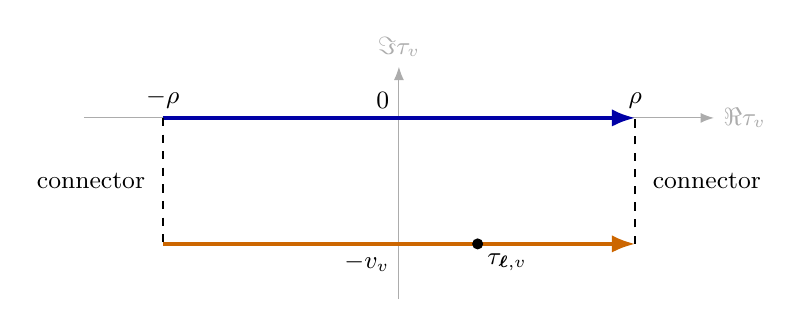
\begin{tikzpicture}[x=1cm,y=1cm,>=Latex,
 every node/.style={font=\small}]
 \draw[->,gray!65] (-4,0)--(4,0) node[right] {$\Re\tau_v$};
 \draw[->,gray!65] (0,-2.3)--(0,.65) node[above] {$\Im\tau_v$};
 \draw[very thick,blue!65!black,->] (-3,0)--(3,0);
 \draw[very thick,orange!80!black,->] (-3,-1.6)--(3,-1.6);
 \draw[dashed,thick] (-3,0)--(-3,-1.6);
 \draw[dashed,thick] (3,-1.6)--(3,0);
 \node[above] at(-3,0){$-\rho$};
 \node[above] at(3,0){$\rho$};
 \node[above left] at(0,0){$0$};
 \fill (1.0,-1.6) circle(2pt);
 \node[below right] at(1,-1.6){$\tau_{\boldsymbol\ell,v}$};
 \node[left] at(-3.1,-.8){connector};
 \node[right] at(3.1,-.8){connector};
 \node[below left] at(0,-1.6){$-v_v$};
\end{tikzpicture}

\caption{One coordinate of the finite angular deformation.
The real box has endpoints \(\pm\rho\), with \(\rho=1/8\);
its translated horizontal side passes through the critical point.
The two vertical sides are retained as connectors, with their
boundary orientations when comparing the horizontal integrals.
Here \(v_v=-\Im\tau_{\boldsymbol\ell,v}>0\).
Other coordinates can have intermediate downward displacements,
so their negative Fourier terms are kept in
\eqref{cta:connector}. The earlier infinite-charge estimate
uses real or translated-grid spectators, before this deformation.}
\label{cta:contour-figure}
\end{figure}

\subsection{Matching the geometric branch}
The analytic action is exactly the action of
\cite[Theorem~1.1]{Geometry}, not just a function with its
complete Hessian. Its derivative \eqref{cta:psi-definition}
agrees on every edge with that theorem, and the constants agree:
\(2G_0=v_{\rm oct}/\pi\), where \(v_{\rm oct}\) is the regular
ideal octahedron volume. This last equality also follows directly
from the Lobachevsky integral at \(\pi/4\).

Write \(n_v=\epsilon_v-2p_v\), with the retained parity
\(\epsilon_v\in\{-1,0,1\}\) in each actual disk frame.
The geometric theorem fills the original primitive slope
\(\mu_v+p_v\lambda_v\), with periods
\[
 U_v=-2\pi\Psi_{\tau_v}-\ii\epsilon_v\tau_v,\qquad
 V_v=2\ii\tau_v.
\]
Its unit-charge equation is
\(\Psi_{\tau_v}+\ii n_v\tau_v/(2\pi)=\ii\), precisely
\eqref{cta:fixedpoint} for \(\boldsymbol\ell=\mathbf1\).
The summed condition implies
\(\sqrt{d_v^2+n_v^2}\ge2^{25/2}>630\).
Furthermore \eqref{cta:tau-formula} gives
\[
 |\tau_{*,v}|\le
 \frac{2\pi}{(1-\delta)\sqrt{d_v^2+n_v^2}}<10^{-2}.
\]
Thus our critical point lies in the geometric theorem's
uniqueness chart. Its original filled metric is smooth,
complete and finite-volume, including zero powers at high-degree
vertices; every main cusp stays complete. Its absolute
fundamental-chain calculation gives
\(\Vol(S^3\setminus K_{\mathbf n})=2\pi\Rea\calC(\mathbf1)\).
There is no appeal here to a long-twist theorem for a zero
power, or to a formal exponentiated slope without metric completion.
Taking logarithms of the already nonzero
\eqref{cta:leading} proves Theorem~\ref{cta:main}.

\subsection{The centered main-meridian insertion}
The finite scalar ledger of \cite[Proposition~8.1]{Meridian}
separates exactly \(A_N(s)\) from the index-dependent factors
\(H_N/W_k\), the shifted crossing grids and the single closing
factor \(H_N(s)\). In the first-charge coefficient every grid
parameter has disappeared because \(c_{1,N}(\sigma)=1\).
The chirp has no remaining \(\sigma\)-dependence once its
recorded scalar is extracted.

It remains to integrate the second line of
\eqref{cta:packet-expansion} on the same joint contour.
For any fixed holomorphic insertion \(h(\boldsymbol\tau)\),
the normalized angular Gaussian evaluates it as
\(h(\boldsymbol\tau_*)+O(N^{-1})\): its linear Gaussian
term vanishes, and the quadratic term and its interaction
with the cubic phase contribute \(O(N^{-1})\).
The expansion to the next order and the fixed losses above
make this statement uniform on \(|s|\le R\).
Apply it to
\(-\pi s^2\sum_e\cot(\pi x_e(\boldsymbol\tau))\),
which already has the factor \(N^{-1}\).
The common first saddle correction cancels upon division
by \(F_N(1)\). The result is \eqref{cta:profile-formula}
with a uniform \(O_R(N^{-2})\) remainder.
In particular the wire values are those at the filled
critical point, not the complete values \(1/4\).

Both \(A_N\) and \(H_N\) are nonzero and bounded away from
zero on the fixed disk for large \(N\).
The ratio in \eqref{cta:profile-formula} tends uniformly
to one. This proves uniform eventual nonvanishing and
the remaining assertions of Theorem~\ref{cta:profile}.
No division by an unproved nonzero finite invariant was
used to establish the leading term.

\section{Scope, dependencies and reproducibility}

The condition is a theorem about every fixed literal marked
tree satisfying \eqref{cta:sum}. It is not uniform in a tree
growing with \(N\), and it is not a condition solely on the
smallest crossing power. For example, in a star with \(d\)
terminal vertices, central power zero and terminal powers \(n\),
\[
 \mathfrak S=\frac1d+\frac{d}{1+n^2}.
\]
Taking \(d\ge2^{27}\) and \(|n|\ge\sqrt{2^{27}d}\) gives
\(\mathfrak S\le2^{-26}\). Knot applicability still requires
the literal endpoint condition of Section~\ref{cta:intro};
this arithmetic example does not supply that condition by itself.
The proof uses neither the separate directed-message criterion
nor the more general strict Conway grammar with bare junctions.

The mathematical dependencies have different jobs.
The finite meridian calculus supplies the exact original
invariant and all repeated-root data.
The factorial lemma supplies one normalized holomorphic
interpolant, and its application to this finite edge sum is
proved in Section~\ref{cta:edge}.
Sections~\ref{cta:angular}--\ref{cta:Fourier} prove the joint
summed-condition analytic estimate, including the entire
original source and Fourier period.
Only after noncancellation is proved is the classical
circle-tree theorem used to identify the action with metric
volume. No quantum asymptotic is an input to that geometric
theorem.

The residue and Gaussian steps belong to the classical
contour method; \cite[Sections~2.4(iii)--(iv)]{DLMF} gives
background. Their contours and all losses relevant to this
finite invariant have been specified above.
From the repository root the paper-local reproduction command is
\begin{verbatim}
python3 papers/circle-tree-asymptotics/check.py \
    --output /tmp/circle-tree-check.json
\end{verbatim}
It records source hashes and reuses the existing edge script's four
exact symbolic identities and finite complex-product samples.
It also checks the numerical budgets by exact rational interval
arithmetic, using convergent series bounds for \(\pi\), \(\sinh\)
and \(\cosh\). Negative controls reject altered budgets.
Those finite calculations do not prove a uniform strip estimate,
the charge tails or a volume theorem; the corresponding
proofs are given here. The script and its recorded result are
linked in the accompanying repository.

\begin{thebibliography}{9}
\bibitem{Meridian}
\emph{Exact Newton calculus for tangles with a moving meridian},
companion paper, Proposition~6.1, Theorem~7.1,
and Proposition~8.1.
\href{https://sashakolpakov.github.io/murakamis_dream/papers/meridian-tangles.pdf}
{Companion PDF}.

\bibitem{Geometry}
\emph{Positive octahedra and primitive fillings for trees of crossing circles},
companion paper, Theorem~1.1.
\href{https://sashakolpakov.github.io/murakamis_dream/papers/circle-tree-geometry.pdf}
{Companion PDF}.

\bibitem{ConwayAnalysis}
\emph{Holomorphic source asymptotics and volume limits for Conway closures},
companion paper, Lemma~2.1.
\href{https://sashakolpakov.github.io/murakamis_dream/papers/conway-asymptotics.pdf}
{Companion PDF}.

\bibitem{Oscillatory}
\emph{Oscillatory filling sums with independently long twists},
companion paper.
\href{https://sashakolpakov.github.io/murakamis_dream/papers/oscillatory-fillings.pdf}
{Companion PDF}.

\bibitem{DLMF}
NIST Digital Library of Mathematical Functions,
\href{https://dlmf.nist.gov/5.11}{Section~5.11, Gamma-function asymptotics},
and \href{https://dlmf.nist.gov/2.4}{Section~2.4, Contour integrals}.
\end{thebibliography}

\end{document}
